\documentclass{beamer}

\mode<presentation> {

%\usetheme{default}
%\usetheme{AnnArbor}
%\usetheme{Antibes}
%\usetheme{Bergen}
%\usetheme{Berkeley}
%\usetheme{Berlin}
% \usetheme{Boadilla}
\usetheme{CambridgeUS}
%\usetheme{Copenhagen}
%\usetheme{Darmstadt}
%\usetheme{Dresden}
%\usetheme{Frankfurt}
%\usetheme{Goettingen}
%\usetheme{Hannover}
%\usetheme{Ilmenau}
%\usetheme{JuanLesPins}
%\usetheme{Luebeck}
% \usetheme{Madrid}
%\usetheme{Malmoe}
%\usetheme{Marburg}
%\usetheme{Montpellier}
%\usetheme{PaloAlto}
%\usetheme{Pittsburgh}
%\usetheme{Rochester}
%\usetheme{Singapore}
%\usetheme{Szeged}
%\usetheme{Warsaw}

%\usecolortheme{albatross}
%\usecolortheme{beaver}
%\usecolortheme{beetle}
%\usecolortheme{crane}
%\usecolortheme{dolphin}
%\usecolortheme{dove}
%\usecolortheme{fly}
%\usecolortheme{lily}
%\usecolortheme{orchid}
%\usecolortheme{rose}
%\usecolortheme{seagull}
%\usecolortheme{seahorse}
%\usecolortheme{whale}
%\usecolortheme{wolverine}

%\setbeamertemplate{footline} % To remove the footer line in all slides uncomment this line
\setbeamertemplate{footline}[page number] % To replace the footer line in all slides with a simple slide count uncomment this line

\setbeamertemplate{navigation symbols}{} % To remove the navigation symbols from the bottom of all slides uncomment this line
}

\usepackage{graphicx}
\usepackage{booktabs} % Allows the use of \toprule, \midrule and \bottomrule in tables

%-------------------------------------------------------------------------------
%	TITLE PAGE
%-------------------------------------------------------------------------------

\title[Short title]{Evaluation of validity of verification methods}

\author{Oskar Ingemarsson, Sebastian Weddmark Olsson}
% \institute[CTH] % Your institution as it will appear on the bottom of every slide, may be shorthand to save space
% {
% Chalmers Tekniska H�gskola, Mecel AB \\ % Your institution for the title page
% }
\date{\today}

\begin{document}

\begin{frame}
  \titlepage
\end{frame}

\begin{frame}
  \frametitle{Overview}
  \tableofcontents
\end{frame}

%-------------------------------------------------------------------------------
%	PRESENTATION SLIDES
%-------------------------------------------------------------------------------

%================================================
\section{What have we done so far?}
%================================================
%------------------------------------------------
\subsection{Implementation}
%------------------------------------------------

\begin{frame}
\frametitle{Implementation}
\begin{itemize}
  \item Watchdog Manager
  \item Erlang implementation of AUTOSAR
\end{itemize}
\end{frame}

\begin{frame}
\frametitle{How QuickCheck works}
Generators, preconditions, postconditions, changes to model state.
\begin{figure}
  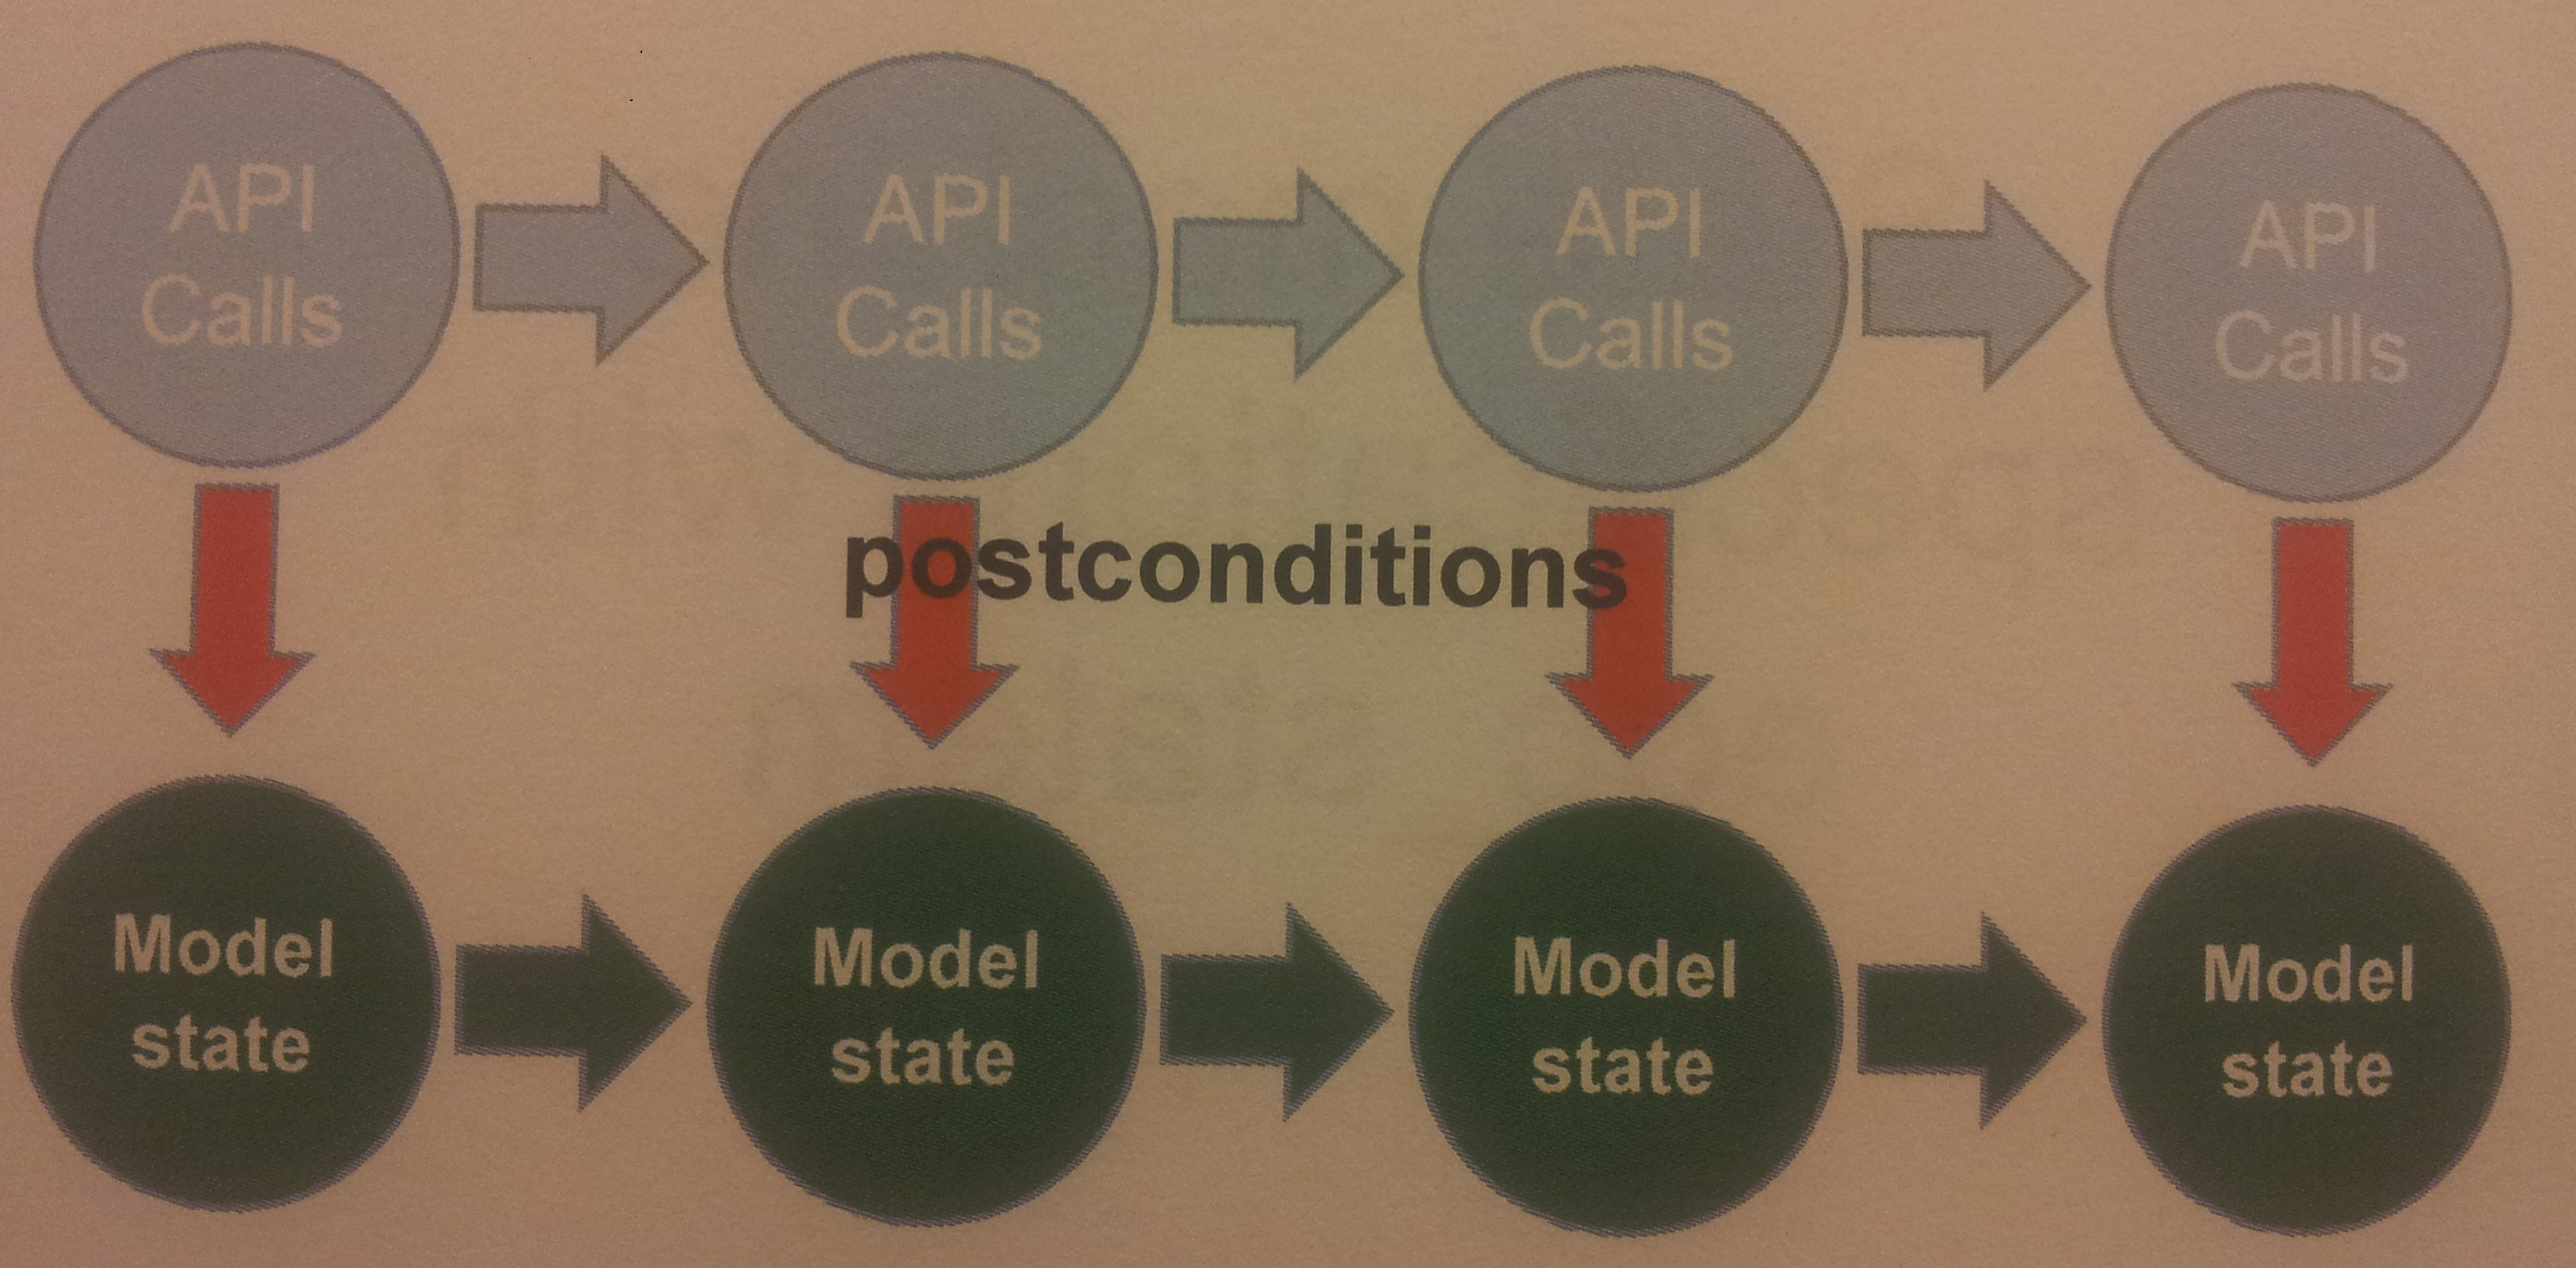
\includegraphics[keepaspectratio, width=0.7\linewidth]{api_calls}
\end{figure}
\end{frame}

\begin{frame}
\frametitle{Example configuration}
Covers most of the model, still quite small.\\
DevErrorDetect is on.\\
\end{frame}

%------------------------------------------------
\subsection{Limitations}
%------------------------------------------------

\begin{frame}
\frametitle{DevErrorDetect}
\begin{itemize}
  \item positive testing
  \item missing requirements
  \item segmentation faults
\end{itemize}
\end{frame}

% %------------------------------------------------
% \subsection{Negative testing}
% %------------------------------------------------

% \begin{frame}
% \frametitle{Red}
% \end{frame}

% %------------------------------------------------
% \subsection{Positive testing}
% %------------------------------------------------

% \begin{frame}
% \frametitle{Green}
% \end{frame}

%------------------------------------------------
\subsection{Tweaking the generators}
%------------------------------------------------

\begin{frame}
\frametitle{What test cases are interesting?}
\begin{itemize}
  \item Negative testing
    \begin{itemize}
      \item good to cover bad arguments
    \end{itemize}
  \item Positive testing
    \begin{itemize}
      \item No absorbing state
      \item correct arguments
      \item correct command sequences
    \end{itemize}
\end{itemize}
\end{frame}

\begin{frame}
\begin{figure}
  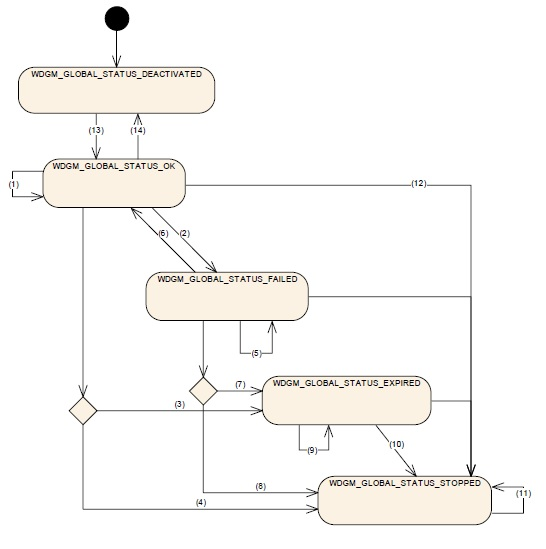
\includegraphics[keepaspectratio, width=0.7\linewidth]{globalstatuses}
\end{figure}
\end{frame}

%================================================
\section{How we handle bugs}
%================================================
%------------------------------------------------
%\subsection{Less good methods}
%------------------------------------------------

\begin{frame}
\frametitle{Less good methods}
\begin{block}{Report bug}
  \begin{description}
    \item[+] Not our job to correct the code
    \item[-] Unknown time delay, probably weeks...
  \end{description}
\end{block}

\begin{block}{Skip the function with the bug}
  \begin{description}
    \item[+] We can continue testing
    \item[-] After finding some bugs, we don't have anything to test at all
  \end{description}
\end{block}
\end{frame}

%------------------------------------------------
%\subsection{Good Methods}
%------------------------------------------------

\begin{frame}
\frametitle{Good methods}
\begin{block}{Fix Model}
  \begin{description}
    \item[+] We can continue testing
    \item[-] Cant test c-code from another configuration or updated version etc.
  \end{description}
\end{block}

\begin{block}{Fix C-code}
  \begin{description}
    \item[+] We can continue testing
    \item[-] Need to get knowledge of the structure etc.
  \end{description}
\end{block}

\begin{block}{Mocking}
  \begin{description}
    \item[+] We can continue testing
    \item[-] Need to make a model for how it should work. The pitfall is if we
      implement the mocked function after the state machine.
  \end{description}
\end{block}
\end{frame}

%================================================
\section{The bugs have we found}
%================================================
%------------------------------------------------
%\subsection{C-code}
%------------------------------------------------

\begin{frame}
\frametitle{C-code}
\begin{tabular}{l l}
  Requirement & Our classification\\\hline
  WDGM286 & Medium\\
  WDGM077 & Low-Medium\footnote{\label{footnot:ett} Together their classification is Medium-High}\\
  WDGM117 & Low-Medium$^{\ref{footnot:ett}}$ \\
  WDGM215 & Low-Medium$^{\ref{footnot:ett}}$ \\
  WDGM216 & Low-Medium$^{\ref{footnot:ett}}$ \\
  WDGM219 & Low-Medium$^{\ref{footnot:ett}}$ \\
  WDGM220 & Low-Medium$^{\ref{footnot:ett}}$ \\
  WDGM182 & High\\
  7.2.3.2 & Medium\footnote{\label{footnot:tva} Together with WDGM252 and WDGM274
    this could be dangerous}\\
  WDGM255 & Low\\
  fig. 4  & Low
\end{tabular}
\end{frame}

%------------------------------------------------
%\subsection{Generated C-code}
%------------------------------------------------

\begin{frame}
\frametitle{Generated C-code and include-files}
\begin{tabular}{l l}
  Requirement & Our classification\\\hline
  p. 27   & Low\\
  fig. 4  & Low\\
\end{tabular}
\end{frame}

%------------------------------------------------
%\subsection{AUTOSAR}
%------------------------------------------------

\begin{frame}
\frametitle{AUTOSAR}
AUTOSAR complications
\begin{itemize}
  \item ambiguous meaning
  \item conflicting requirements
  \item omitted requirements/explanations
  \item spelling of configuration parameters
  \item references
\end{itemize}
\end{frame}

%================================================
\section{Testing}
%================================================
%------------------------------------------------
%\subsection{Coverage}
%------------------------------------------------

\begin{frame}
\frametitle{Coverage}
%if our model behave like the c model, then we can test our models function
%coverage and check that we test all functions.
\begin{itemize}
  \item line coverage analysis (not absolute, due to bugs in C-code)
  \item variables in the state
  \item call coverage (not absolute)
\end{itemize}
\end{frame}

%------------------------------------------------
%\subsection{Statistics}
%------------------------------------------------

\begin{frame}[fragile]
\frametitle{Statistics}
\begin{itemize}
  \item generated command sequences of up to 120 commands (really no limit)
  \item 95\% starts with the command \verb!WdgM_Init!
  \item global statuses
%% kanske h�r mer till implementationen men vi borde n�mna procentsatser p�
%% globalstatusar kanske?
  % \item There is five global statuses, a functional system initiates to
  %   \verb!WDGM_GLOBAL_STATUS_DEACTIVATED!, and if the command
  %   \verb!WdgM_Init! is successfully called, the global status should be
  %   \verb!WDGM_GLOBAL_STATUS_OK!. After that, only the commands
  %   \verb!WdgM_Mainfunction! and \verb!WdgM_DeInit! can change the global
  %   status.
\end{itemize}
\end{frame}

\begin{frame}
\begin{figure}
  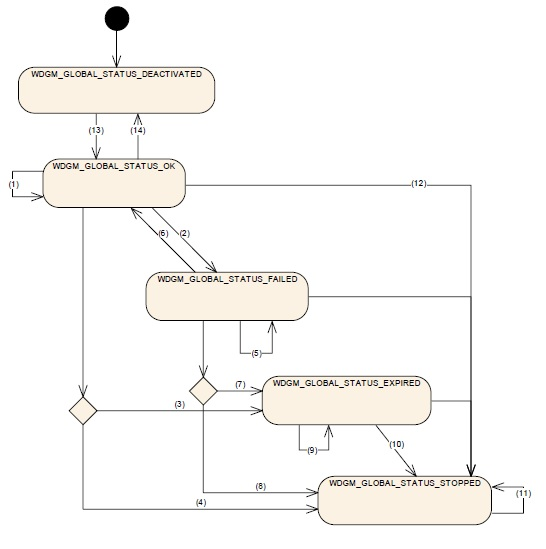
\includegraphics[keepaspectratio, width=0.7\linewidth]{globalstatuses}
\end{figure}
\end{frame}

%------------------------------------------------
%\subsection{Suitable tests}
%------------------------------------------------

\begin{frame}[fragile]
\frametitle{Suitability of tests}
We generate lists of commands, most of which starts with \verb!WdgM_Init! or it has
\verb!WdgM_Init! in the first 2-4 commands. This is a precondition for all other
functions except \verb!WdgM_GetFirstExpiredSEId!.\\[0.5cm]

The functions that change the state considerably is
\verb!WdgM_Checkpointreached!, \verb!WdgM_SetMode! and \verb!WdgM_Mainfunction!.
Therefor we prioritize these functions in the generation.
\end{frame}

%================================================
\section{Future work}
%================================================

\begin{frame}[fragile]
\frametitle{Functional Safety}
We will look at how this testing suites ISO26262. We have good hopes of
achieving some kind of classification.\\[0.5cm]

When the configuration flag \verb!DevErrorDetect! is off, you may get
segmentation faults.
% When the configuration flag \verb!DevErrorDetect! is off, and you send a
% null pointer to \verb!WdgM_Init! you get a segmentation fault.
\end{frame}

\begin{frame}
\frametitle{Bug report}
As stated, we have found a lot of bugs and we have modified the C-code.
\end{frame}

\begin{frame}
\frametitle{Shrinking....}
We found out that there is some problems when QuickCheck tries to shrink failed
tests. This is because most of the commands we send in depend on the state, and
QuickCheck just tries to shrink the generated commands/arguments. Many of which
will fail because some other (previous) command has been neglected.\\[0.5cm]

It is possible to guide QuickCheck to shrink correctly, but it wont be a part of
this thesis, because time.
\end{frame}

\begin{frame}[fragile]
\frametitle{Combining modules}
Another part of future work could be to implement a model for \verb!WdgIf! and
get the two modules to work coherently.
\end{frame}
%------------------------------------------------

% \begin{frame}
% \frametitle{Kolumner}
% \begin{columns}[c]
% \column{.45\textwidth}
% v�nster
% \column{.5\textwidth}
% h�ger
% \end{columns}
% \end{frame}

% \begin{frame}[fragile] % Need to use the fragile option when verbatim is used in the slide
% \frametitle{Verbatim}
% \begin{example}[Theorem Slide Code]
% \begin{verbatim}
% Code
% \end{verbatim}
% \end{example}
% \end{frame}

% \begin{frame}
% \frametitle{Figure}
% %\begin{figure}
% %\includegraphics[width=0.8\linewidth]{test}
% %\end{figure}
% \end{frame}


%================================================
\section{Questions}
%================================================

\begin{frame}
\Huge{\centerline{Questions?}}
\end{frame}

%-------------------------------------------------------------------------------

\begin{frame}
\frametitle{Estimated time}
\begin{columns}[c]
  \column{.5\textwidth}
  \begin{tabular}{l l}
    Reading (and under-\\standing)
    AUTOSAR & 4 weeks\\
    Understanding C-code & 2 week\\
    Implementing model & 3 weeks\\
    Testing & over time\\
    Tweaking & 2 weeks
  \end{tabular}

  \column{.45\textwidth}
  Most off these items has a continuous work and we have done the work in an
  iterative way.
\end{columns}
\end{frame}

%-------------------------------------------------------------------------------

\end{document}